\chapter{Frontend Architecture and User Manual}

\section{Technology Choices}
\subsection{Flutter}
We chose \textbf{Flutter} as the frontend framework due to its:
\begin{itemize}
    \item Cross-platform capabilities
    \item High-performance rendering engine (Skia)
    \item Rich widget ecosystem
    \item Strong Material 3 and community support
\end{itemize}

\subsection{Dart}
Dart provides AOT compilation and a simple async model, ideal for UI-driven apps.

\subsection{Provider (State Management)}
Used for lightweight, app-wide state handling (e.g., tokens, theme, user info).

\subsection{flutter\_markdown}
Renders AI-generated content with headers, bold, lists, and emphasis.

\subsection{Syncfusion Charts}
Professional, animated charts used for contract visualizations.

\subsection{Firebase Auth}
Handles user authentication, offloading token validation to the backend.

\section{Workflow Overview}

\begin{figure}[H]
    \centering
    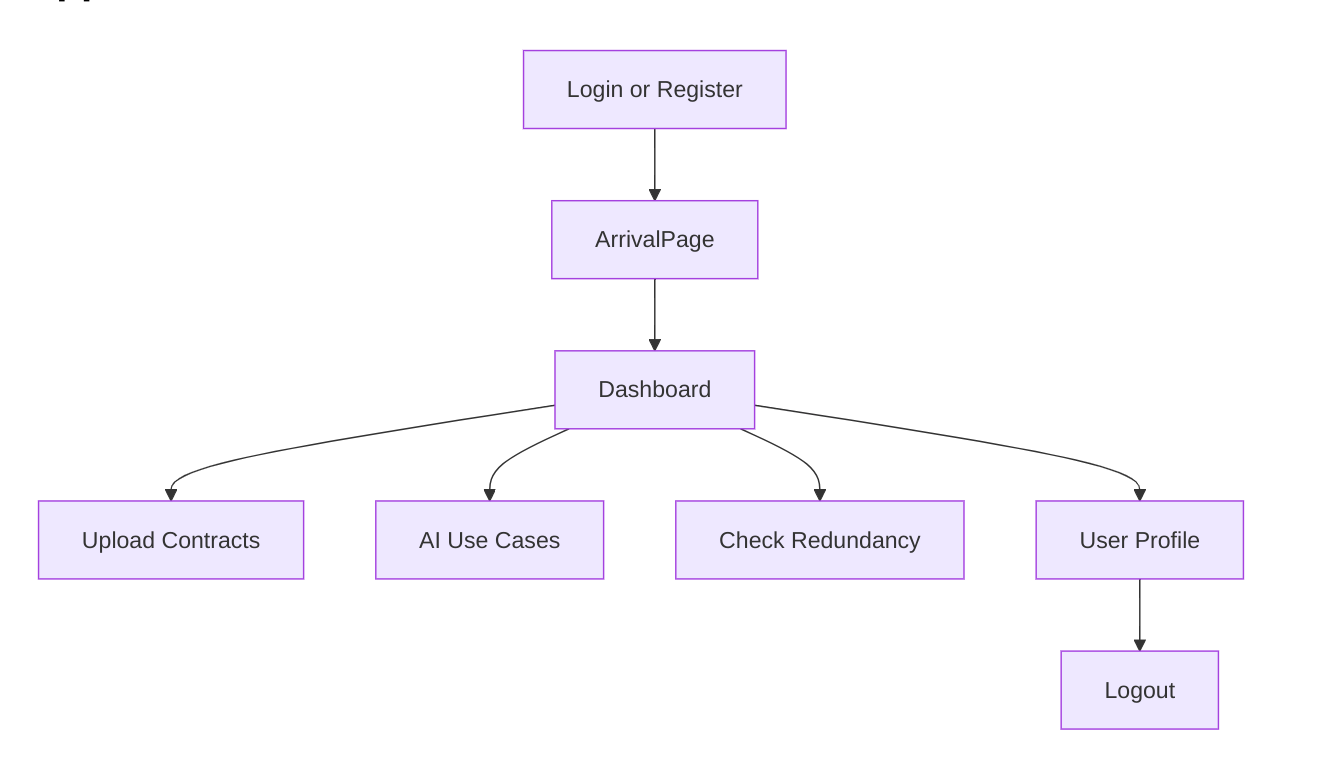
\includegraphics[width=0.8\textwidth]{frontend/workflow_mermaid.png}
    \caption{Frontend workflow from login to dashboard and feature pages}
\end{figure}

\section{Project Structure}

\begin{verbatim}
lib/
├── main.dart
├── http_client.dart
├── pages/
│   ├── auth_page.dart
│   ├── register_page.dart
│   ├── arrival_page.dart
│   ├── home.dart
│   ├── upload_contract_page.dart
│   ├── usecaseun_page.dart
│   ├── usecasedeux_page.dart
│   ├── user_profile.dart
│   ├── side_menu.dart
│   └── navigation_page.dart
├── providers/
│   └── app_state.dart
├── widgets/
│   ├── custom_app_bar.dart
│   └── navbar.dart
\end{verbatim}

\section{Component Highlights}

\textbf{main.dart:} Initializes the app, theme, routing and Provider.\\
\textbf{http\_client.dart:} Authenticated API wrapper.\\
\textbf{app\_state.dart:} Global state (token, theme, user info).\\
\textbf{home.dart:} Dashboard with Syncfusion pie charts and Markdown summaries.

\section{User Manual}

\subsection*{Step 1: Login / Register}

\begin{figure}[H]
    \centering
    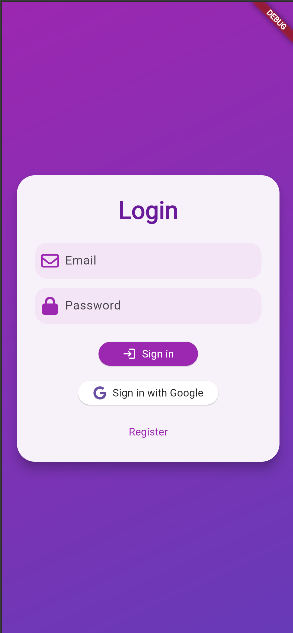
\includegraphics[width=0.4\textwidth]{frontend/login.png}
    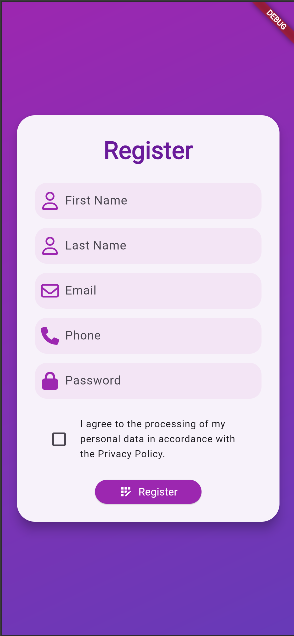
\includegraphics[width=0.4\textwidth]{frontend/register.png}
    \caption{Login and registration pages}
\end{figure}

\subsection*{Step 2: Explore Dashboard}

\begin{figure}[H]
    \centering
    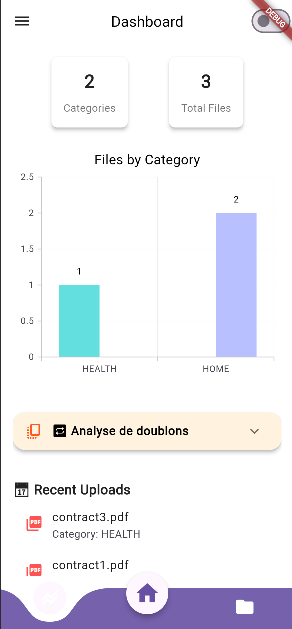
\includegraphics[width=0.45\textwidth]{frontend/dashboard_ui.png}
    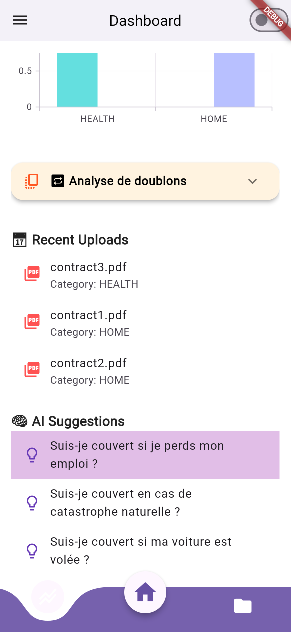
\includegraphics[width=0.45\textwidth]{frontend/dashboard_ui2.png}
    \caption{Dashboard with charts and AI insights}
\end{figure}

\subsection*{Step 3: Upload Documents}

\begin{figure}[H]
    \centering
    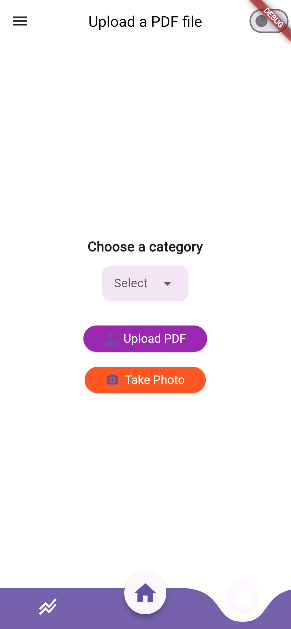
\includegraphics[width=0.5\textwidth]{frontend/upload_contract.png}
    \caption{Upload screen with file picker and category selector}
\end{figure}

\subsection*{Step 4: Use the AI Assistant}

\begin{figure}[H]
    \centering
    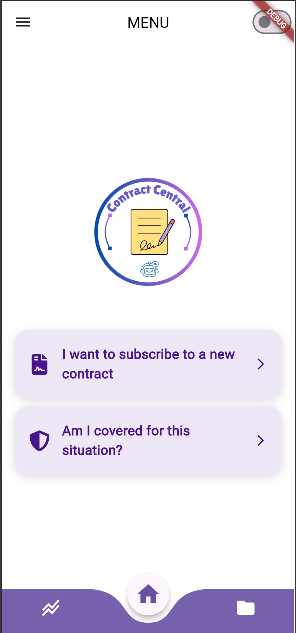
\includegraphics[width=0.45\textwidth]{frontend/menu.png}
    \hspace{0.05\textwidth}
    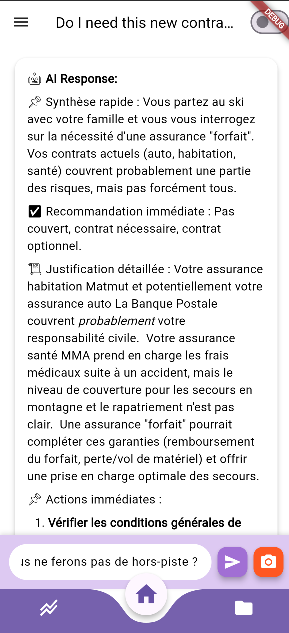
\includegraphics[width=0.45\textwidth]{frontend/usecase_1.png}
    \caption{Use case menu and AI question screen}
\end{figure}

\newpage

\begin{figure}[H]
    \centering
    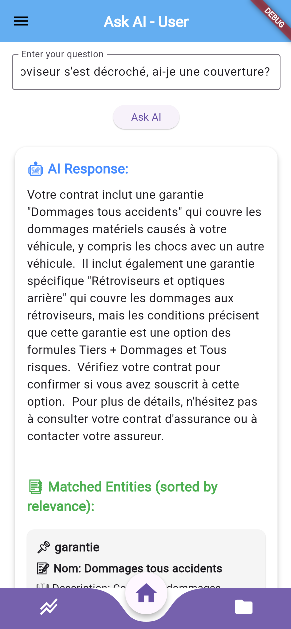
\includegraphics[width=0.45\textwidth]{frontend/usecase_2.png}
    \hspace{0.05\textwidth}
    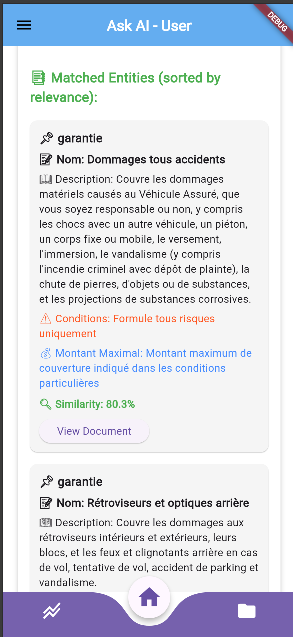
\includegraphics[width=0.45\textwidth]{frontend/usecase_2_photo2.png}
    \caption{AI response and matched clauses display}
\end{figure}


\subsection*{Step 5: Detect Redundancy}

\begin{figure}[H]
    \centering
    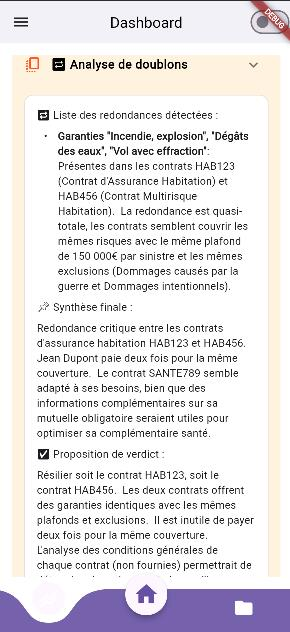
\includegraphics[width=0.6\textwidth]{frontend/dashboard_doublon.png}
    \caption{Redundancy detection view}
\end{figure}

\subsection*{Step 6: Profile and Logout}

\begin{figure}[H]
    \centering
    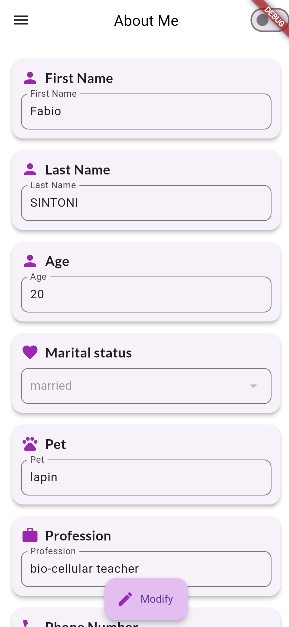
\includegraphics[width=0.5\textwidth]{frontend/profile_page.png}
    \caption{User profile page with logout functionality}
\end{figure}

\subsection*{Step 7: Dark Mode}

\begin{figure}[H]
    \centering
    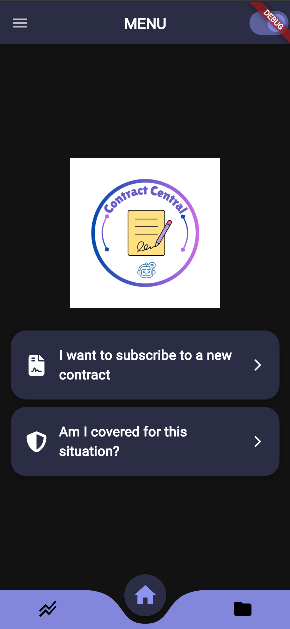
\includegraphics[width=0.4\textwidth]{frontend/dark_mode_toggle.png}
    \caption{Dark/light theme toggle}
\end{figure}

\subsection*{Step 8: Navigation}

\begin{figure}[H]
    \centering
    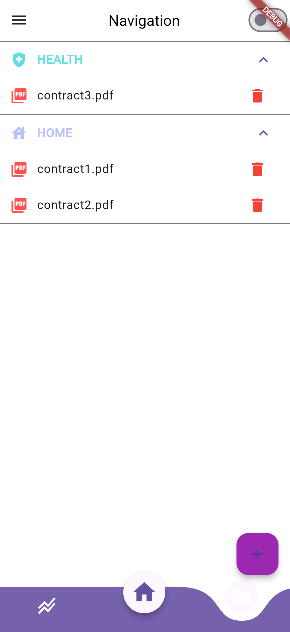
\includegraphics[width=0.4\textwidth]{frontend/navigation_menu.png}
    \caption{Side navigation drawer and menu button}
\end{figure}

\section*{Summary}

Contract Central's frontend is designed with performance and clarity in mind. Thanks to Flutter, it offers smooth navigation, AI integration, and clear contract visualization across platforms.
